\section{Study Settings}

In this section, we present the setting of our study, whose main goal is to perform a non-exact replication of the work of Bao et al. and understand the implications of static analysis algorithms in his results. We also investigate how static analysis can improve the performance of mining sandboxes, in the task of identifying malicious behaviors.

To achieve these general goals, we intend to answer the following research questions.

\begin{enumerate}[(RQ1)]
\item What is the impact of static analysis DroidFax at the Bao et al. study ?
\item What is the effective performance of each test generation tool, in terms of the number of detected malware, at Bao et al work, disregarding static analysis DroidFax ?
\item What benefits of using tainted analysis algorithms to complement the dynamic analysis provided by test generation tools, for mining sandboxes ?
\end{enumerate}

Answering these research questions has several implications. The questions (RQ1) and (RQ2) for instance, can disclose an overestimation of the performance of test generation tools for mining sandboxes, explored at Bao et al work, and introduce a possible threat to the final work conclusions. Lastly, the third research question allows us to open up the possibility of finding new strategies for improving the technique of mining sandboxes, strengthening the static analysis, through the use of tainted analysis algorithms.

We conducted two studies to answer the research questions above. First we performed a non-exact replication of Bao et al work. For that purpose, we initially selected four test generation tools, three from the original study, and other recently proposed. The original test generation tools used were: Droidbot (academic) \cite{DBLP:conf/icse/LiYGC17}, DroidMate  (academic) \cite{DBLP:conf/icse/JamrozikZ16} and Monkey (industry) \cite{Monkey}. Droidbot and DroiMate were selected because, at original study, they achieved the best performance on detecting malicious behavior at their respective sandboxes. We also select Monkey because it is the main and the most popular test generation tool used by Android developers, coming up with Android SDK installation. The other test generation tool selected was Humanoid (academic) \cite{DBLP:conf/kbse/LiY0C19}, a recent test generation tool, that generates human-like test inputs using deep learning techniques, promising to achieve higher and faster code coverage than state-of-the-art test generation tool. 

For this non-exact replication, we also used a benchmark called droidXP \cite{DBLP:conf/scam/CostaMCMVBC20}. The benchmark helps us to reproduce the original work, allowing integrate test generation tools, define execution time for each tool, and the number of study repetitions. The droidXP benchmark relies on DroidFax, the same tool used by Bao et al. in your study. Droidfax instrumented Android apps and collected relevant information about their execution (using the test case generation tools). It collects the set of sensitive APIs accessed during test execution, and during static analysis at instrumentation stage of each app. Based on these sensitive APIs access, the sandbox of each tool will be compose. For this study we considered two metrics: The number of malware that each test generation tool detected, and the code coverage of each tool at the analysis time.  

The second study, we used a static taint analysis approaches through Flowdroid \cite{DBLP:conf/pldi/ArztRFBBKTOM14} tool, that execute this kind of analysis at Android apps. Our aim is to investigate the performance on detecting malicious behavior using static taint analysis at Android apps. The metrics computed at this study was the number of source-sink flows at pairs apps (B/M), and analysis time at each apps.

At both studies, we employed the same dataset, 98 pair of real-world apps (B/M), shared by the AndroZoo \cite{DBLP:conf/msr/AllixBKT16} group. We detail the procedures of each study in what follows.

\subsection{First Study: A non-exact replication}

In this first study, we executed droidXP benchmark with your default configuration, that is, using static analysis Droidfax and test generation tools while collecting the accessed sensitive APIs. We investigate the four test case generation tools described earlier and added a fifth tool described as Joke tool. Joke is a ``fake" tool that simulates a test tool that does nothing during the benchmark execution. Using this tool, the results of the dynamic analysis are not considered and we can compute the results with only the static analysis, performed by Droidfax. Our study executed each pairs app (B/M) in each one of the five test generator tool, including Joke, for three minutes, and for just one time. We investigate the capacity to detect malicious behaviors in the corresponding malign app by the sandbox, modeled by test generation tool under analysis. (Figure \ref{fig:setup}) show this experimental setup.

\begin{figure}[ht]
  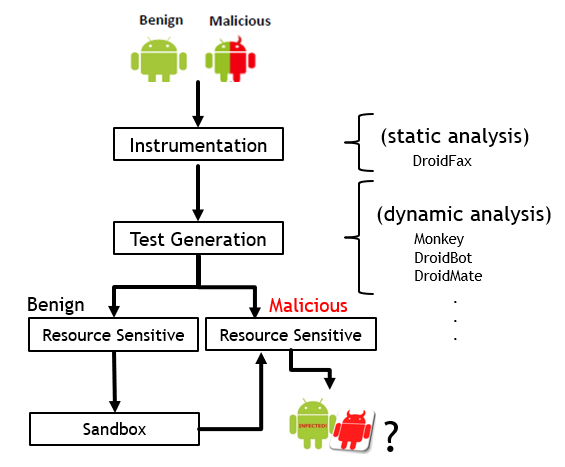
\includegraphics[width=0.45\textwidth]{images/setup.png}
  \label{Experiment setup}
  \caption{Experiment setup}
  \label{fig:setup}
\end{figure}

In a second moment, we used an benchmark option that disables the static analysis performed by DroidFax. With this new configuration, we executed the benchmark again, with the same dataset apps, the same execution time, and the same test case generation tools. With the results, it was possible to compute the real aid portion of the dynamic analysis in the malware detection of each test generation tool, since the results, was computed without the static analysis Droidfax influence.

We used this study to answer the research questions (RQ1) and (RQ2), since the ``fake" tool result, presented the real impact of static analysis on benchmark, assuming that Joke tool, do not performs dynamic analysis, depending solely Droidfax static analysis to detect malicious behaviors.


\subsection{Second Study: Tainted analysis algorithms.}

To complement our initial study, we performed the tainted analysis at the same data set from the first study. For this second study, we used a static flow analysis tool for Android apps, called Flowdroid \cite{10.1145/2666356.2594299}. The goal is to test accuracy of static analysis, through tainted analysis algorithms, at finding malicious behavior, and compare the results with previous study at the same data set. At this second study, a behavior is considered malicious, every time the algorithms detected a flow suspicious, between source and sink, that can characterize a privacy leaks.

Initially, Flowdroid mine all sources and sinks of each benign apps, and enumerates all possible data flows between them. Next, it performs the same process for the malicious app correspondent. In the final step, we compared the set of source-sink track between the benign app and its corresponding malicious app, in order to discovery some taint tracer different between the apps under analysis.

This study was useful to answer the research question (RQ3), because it disclosed some pairs of applications with malicious behavior, that could not be detected at first study at none of the scenarios presented, evidencing that there is a benefit of new static analysis techniques, to complement the dynamic analysis provided by test generation tools, at mining sandboxes solutions. Details of studies results are at next section.





